\documentclass{article}
\usepackage[utf8]{inputenc}
\usepackage{listings}
\usepackage{graphicx}
\usepackage{float}
\usepackage{xcolor}
\usepackage{geometry}
\usepackage{CJKutf8}
\usepackage{amsmath}
\usepackage{amssymb}

\geometry{a4paper,scale=0.8}
\lstset{
    basicstyle          =   \sffamily,        
    keywordstyle        =   \bfseries,         
    commentstyle        =   \rmfamily\itshape, 
    stringstyle         =   \ttfamily, 
    flexiblecolumns,               
    numbers             =   left,  
    showspaces          =   false, 
    showstringspaces    =   false,
    captionpos          =   t,     
    frame               =   lrtb, 
}

\lstdefinestyle{Python}{
    language        =   Python, % 语言选Python
    basicstyle      =   \zihao{-5}\ttfamily,
    numberstyle     =   \zihao{-5}\ttfamily,
    keywordstyle    =   \color{blue},
    keywordstyle    =   [2] \color{teal},
    stringstyle     =   \color{magenta},
    commentstyle    =   \color{red}\ttfamily,
    breaklines      =   true,  
    columns         =   fixed,  
    basewidth       =   0.5em,
}

\title{\bf\Large  概率论与数理统计 第9次作业}
%%%%%%%%%%%%%%%%%%%%%%%%%%%%%%%%%%%%%%
%% DON'T forget to change this part %%
\author{\bf Name: 宋昊原 \qquad Student ID: 2022010755}
%%%%%%%%%%%%%%%%%%%%%%%%%%%%%%%%%%%%%%

\begin{document}
\begin{CJK}{UTF8}{gbsn}
\maketitle
\section{概率知识总结}
\begin{itemize}
    \item 事件的概率
    \begin{itemize}
        \item 事件、事件的运算
        \item 概率的三种解释
        \begin{itemize}
            \item 古典解释
            \item 频率解释
            \item 主观解释
        \end{itemize}
        \item 概率的公理化定义
        \item 条件概率
        \item 事件的独立性
        \item Bayes公式
    \end{itemize}
    \item 随机变量
    \begin{itemize}
        \item 累积分布函数
        \item 离散型随机变量和概率质量函数
        \begin{itemize}
            \item Bernoulli分布
            \item 二项分布
            \item Poisson分布
        \end{itemize}
        \item 连续型随机变量和概率密度函数
        \begin{itemize}
            \item 均匀分布
            \item 正态分布
            \item 指数分布
        \end{itemize}
        \item 随机变量的函数
    \end{itemize}
    \item 随机向量
    \begin{itemize}
        \item 联合累积分布函数
        \item 离散分布和联合概率质量函数
        \begin{itemize}
            \item 多项分布
        \end{itemize}
        \item 连续分布和联合概率密度函数
        \begin{itemize}
            \item 二元正态分布
        \end{itemize}
        \item 边际分布
        \item 条件分布和随机变量的独立性
        \item 随机向量的函数
        \begin{itemize}
            \item 直接求解函数的分布
            \item 密度函数变换法
        \end{itemize}
    \end{itemize}
    \item 随机变量的数字特征
    \begin{itemize}
        \item 期望
        \item 分位数
        \item 方差、标准差
        \item 协方差、相关系数
        \item 矩、偏度系数、峰度系数
        \item 矩母函数
        \begin{itemize}
            \item 矩母函数和矩的关系
            \item 矩母函数确定分布
        \end{itemize}
        \item 条件期望和全期望公式
    \end{itemize}
    \item 概率不等式与极限定理
    \begin{itemize}
        \item 概率不等式
        \begin{itemize}
            \item Markov不等式
            \item Chebishev不等式
            \item Chernoff不等式
        \end{itemize}
        \item 随机变量列的收敛性
        \begin{itemize}
            \item 依概率收敛
            \item 以概率1收敛
            \item 依分布收敛
        \end{itemize}
        \item 极限定理
        \begin{itemize}
            \item Khinchin弱大数定律
            \item Kolmogrov强大数定律
            \item 中心极限定理
        \end{itemize}
    \end{itemize}
\end{itemize}
主要问题在于期望方差的证明、随机变量列收敛的证明等证明题的思路.
\section{抽样调查案例}
高中数学课统计单元曾布置过一个作业,要求调查关于高考3+3选科方案的内容. 然而,我们抽样的方式采取发朋友圈的方便抽样的方式,由于课程关联、分班等原因,我们认识的同学中选择理科的比例要比年级里高得多,这样的抽样很可能不具备代表性.
\section{简单随机抽样}
\subsection{}
只需证明$X_{i}$取得总体中任何一个选择$x_{j}$的概率确实是$\frac{1}{N}$即可.
$$ P(X_{i}=x_{j})=P(X_{1}\neq x_{j}\land ...\land X_{i-1}\neq x_{j})P(X_{i}=x_{j}|X_{1}\neq x_{j}\land...\land X_{i-1}\neq x_{j})$$
$$ =\frac{N-1}{N}\times\frac{N-2}{N-1}\times ... \times\frac{N-i+1}{N-i+2}\times\frac{1}{N-i+1}=\frac{1}{N}$$
即所有$X_{i}$同分布,故有
$$ E(X_{i})=\sum\limits_{j=1}^{N}\frac{1}{N}x_{j}=\mu$$
$$ Var(X_{i})=\sum\limits_{j=1}^{N}\frac{1}{N}(x_{j}-\mu)^{2}=\sigma^{2}$$
\subsection{}
$$ E(\bar{X})=\frac{1}{n}\sum\limits_{i=1}^{n}E(X_{i})=\mu$$
$$ E(\bar{X}^{2})=\frac{1}{n^{2}}(\sum\limits_{i=1}^{n}E(X_{i}^{2})+2\sum\limits_{1\leq i<j\leq n}E(X_{i}X_{j}))$$
其中
$$ E(X_{i}^{2})=Var(X_{i})+E^{2}(X_{i})=\mu^{2}+\sigma^{2}$$
$$ E(X_{i}X_{j})=\frac{1}{N(N-1)}(\sum\limits_{1\leq k,l\leq N\land k\neq l}x_{k}x_{l})$$
$$ =\frac{1}{N(N-1)}((\sum\limits_{k=1}^{N}x_{k})^{2}-\sum\limits_{k=1}^{N}x_{k}^{2})$$
$$ =\frac{1}{N(N-1)}(N^{2}\mu^{2}-N(\mu^{2}+\sigma^{2}))$$
$$ =\mu^{2}-\frac{1}{N-1}\sigma^{2}$$
故
$$ E(\bar{X}^{2})=\frac{1}{n^{2}}(n(\mu^{2}+\sigma^{2})+n(n-1)(\mu^{2}-\frac{1}{N-1}\sigma^{2}))$$
$$ =\mu^{2}-\frac{1}{n}(\frac{N-n}{N-1})\sigma^{2}$$
故
$$ Var(\bar{X})=E(\bar{X}^{2})-E^{2}(\bar{X})=\frac{\sigma^{2}}{n}(\frac{N-n}{N-1})$$
\section{二项总体的估计}
\subsection{}
总体的均值为$kp$,方差为$kp(1-p)$,矩估计为
$$ kp\approx \bar{X}$$
$$ kp(1-p)\approx \frac{1}{n}\sum\limits_{i=1}^{n}(X_{i}-\bar{X})^{2}$$
故
$$ p\approx 1-\frac{\sum\limits_{i=1}^{n}(X_{i}-\bar{X})^{2}}{n\bar{X}}$$
$$ k\approx \frac{\bar{X}}{1-\frac{\sum\limits_{i=1}^{n}(X_{i}-\bar{X})^{2}}{n\bar{X}}}=\frac{n\bar{X}^{2}}{n\bar{X}-\sum\limits_{i=1}^{n}(X_{i}-\bar{X})^{2}}$$
\subsection{}
根据第11题计算机实验中的讨论,上述估计在$n$或$p$较小时很不准确.
\section{均匀总体的估计}
\subsection{矩估计}
$$\mu=\frac{3}{2}\theta$$
故
$$\theta\approx\frac{2}{3}\bar{X}$$
\subsection{极大似然估计}
均匀分布的概率密度函数为
\begin{equation}
    f_{1}(x;\theta)=\left\{
    \begin{array}{cl}
    \frac{1}{\theta} & \theta\leq x\leq 2\theta\\
    0 & else\\
    \end{array}\right.
\end{equation}
故似然函数
\begin{equation}
    L(\theta)=\left\{
    \begin{array}{cl}
    \frac{1}{\theta^{n}} & \theta\leq X_{1},...,X_{n}\leq 2\theta\\
    0 & else\\
    \end{array}\right.
\end{equation}
要使$L(\theta)$取最大值,只需在满足$\theta\leq X_{1},...,X_{n}\leq 2\theta$的条件下取最小的$\theta$,即
$$\theta^{*} = \frac{\max\limits_{i}X_{i}}{2}$$
\section{特殊分布的估计}
\subsection{}
显然有$f(x;a,\sigma)\geq0,\forall x\in\mathbb{R}$
$$\int_{-\infty}^{+\infty}f(x;a,\sigma)dx=\frac{1}{\sigma^{2}}\int_{-\infty}^{+\infty}\frac{(x-a)^{2}}{\sqrt{2\pi}\sigma}\exp(-\frac{1}{2\sigma^{2}}(x-a)^{2})dx$$
$$ =\frac{1}{\sigma^{2}}Var(N(a,\sigma^{2}))=1$$
\subsection{矩估计}
总体均值
$$ E(X)=\int_{-\infty}^{+\infty}\frac{x(x-a)^{2}}{\sqrt{2\pi}\sigma^{3}}\exp(-\frac{1}{2\sigma^{2}}(x-a)^{2})dx$$
$$ =\int_{-\infty}^{+\infty}\frac{(x-a)^{3}}{\sqrt{2\pi}\sigma^{3}}\exp(-\frac{1}{2\sigma^{2}}(x-a)^{2})d(x-a)+a\int_{-\infty}^{+\infty}\frac{(x-a)^{2}}{\sqrt{2\pi}\sigma^{3}}\exp(-\frac{1}{2\sigma^{2}}(x-a)^{2})dx$$
$$ =0+a=a$$
总体方差
$$ Var(X)=\int_{-\infty}^{+\infty}\frac{(x-a)^{4}}{\sqrt{2\pi}\sigma^{3}}\exp(-\frac{1}{2\sigma^{2}}(x-a)^{2})dx$$
$$ =\int_{-\infty}^{+\infty}\frac{x^{4}}{\sqrt{2\pi}\sigma^{3}}\exp(-\frac{1}{2\sigma^{2}}x^{2})dx$$
令$\xi = \frac{x}{\sigma}$,有
$$ Var(X)=\int_{-\infty}^{+\infty}\frac{\xi^{4}\sigma^{2}}{\sqrt{\pi}}\exp(-\frac{\xi^{2}}{2})d\xi=3\sqrt{2}\sigma^{2}$$
故
$$ a\approx \bar{X}$$
$$ \sigma^{2} \approx \frac{\sum\limits_{i=1}^{n}(X_{i}-\bar{X})^{2}}{3\sqrt{2}n}$$
\subsection{极大似然估计}
似然函数
$$ L(a,\sigma^{2})=\prod\limits_{i=1}^{n}\frac{(X_{i}-a)^{2}}{\sqrt{2\pi}\sigma^{3}}\exp(-\frac{(X_{i}-a)^{2}}{2\sigma^{2}})$$
故
$$ \ln L(a,\sigma^{2})=\sum\limits_{i=1}^{n}(2\ln|X_{i}-a|-\frac{(X_{i}-a)^{2}}{2\sigma^{2}}-\ln(\sqrt{2\pi}\sigma^{3}))$$
似然方程为
$$ \frac{\partial\ln L(a,\sigma^{2})}{\partial a}=\sum\limits_{i=1}^{n}(-\frac{2}{X_{i}-a}+\frac{X_{i}-a}{\sigma^{2}})=0$$
$$ \frac{\partial\ln L(a,\sigma^{2})}{\partial \sigma^{2}}=\sum\limits_{i=1}^{n}(\frac{(X_{i}-a)^{2}}{2\sigma^{4}}-\frac{3}{2\sigma^{2}})=0$$
即
$$ \sum\limits_{i=1}^{n}\frac{(X_{i}-a)^{2}}{\sigma^{2}}-2n=0$$
$$ \sum\limits_{i=1}^{n}\frac{(X_{i}-a)^{2}}{\sigma^{2}}-3n=0$$
这似乎是个矛盾方程.
% TODO why?
\section{Bernoulli分布估计}
\subsection{矩估计}
$$ p\approx \bar{X}$$
\subsection{极大似然估计}
$$ L(p)=p^{X_{1}+...+X_{n}}(1-p)^{n-X_{1}-...-X_{n}}=p^{n\bar{X}}(1-p)^{n-n\bar{X}}$$
$$ \ln L(p)=n\bar{X}\ln p+n(1-\bar{X})\ln(1-p)$$
令
$$ \frac{\partial\ln p}{\partial p}=\frac{n\bar{X}}{p}-\frac{n(1-\bar{X})}{1-p}=0$$
$$(1-p^{*})\bar{X}=p^{*}(1-\bar{X})$$
$$p^{*}=\bar{X}$$
这确实是最大值点.
\section{多项分布极大似然估计}
联合分布PMF为
$$ L(\mathbf{p})=f(X_{1},...,X_{m};p_{1},...,p_{m})=\frac{n!}{X_{1}!...X_{m}!}p_{1}^{X_{1}}...p_{m}^{X_{m}}$$
$$ \ln L(\mathbf{p})=\ln\frac{n!}{X_{1}!...X_{m}!}+X_{1}\ln p_{1}+...+X_{m}\ln p_{m}$$
需要找此函数在$p_{1}+...+p_{m}=1$条件下的条件极值,故考虑Lagrange函数:
$$ \tilde{L}(\mathbf{p},\lambda)=\ln\frac{n!}{X_{1}!...X_{m}!}+X_{1}\ln p_{1}+...+X_{m}\ln p_{m}+\lambda(p_{1}+...+p_{m}-1)$$
故
$$ \frac{\partial{\ln L(\mathbf{p})}}{\partial(\mathbf{p},\lambda)}=\begin{bmatrix}
    \frac{X_{1}}{p_{1}}+\lambda & ... & \frac{X_{m}}{p_{m}}+\lambda & p_{1}+...+p_{m}-1\end{bmatrix}$$
令上述梯度为$\mathbf{0}$,则有
$$ \frac{X_{1}}{p_{1}}=...=\frac{X_{m}}{p_{m}}=-\lambda$$
$$ p_{1}+...+p_{m}=1$$
故
$$ p_{i}=\frac{X_{i}}{X_{1}+...+X_{m}}$$
这是符合预期的估计.
\section{给定分布的估计}
\subsection{矩估计}
$$ E(X)=\theta^{2}+4\theta(1-\theta)+3(1-\theta)^{2}=3-2\theta$$
此时
$$ \bar{X}=\frac{4}{3}$$
故
$$ \hat{\theta}=\frac{5}{6}$$
\subsection{极大似然估计}
$$ L(\theta)=2\theta^{5}(1-\theta)=2\theta^{5}-\theta^{6}$$
令
$$ \frac{dL(\theta)}{d\theta}=5\theta^{4}-6\theta^{5}=0$$
有
$$ \theta^{*}=\frac{5}{6}$$
这确实是最大值点.
\section{某种幂分布的估计}
\subsection{矩估计}
$$ E(X)=\int_{0}^{1}\theta x^{\theta}dx=\frac{\theta}{\theta+1}$$
故
$$ \frac{\hat{\theta}}{\hat{\theta}+1}=\bar{X}$$
$$ \hat{\theta}=\frac{\bar{X}}{1-\bar{X}}$$
\subsection{极大似然估计}
$$ L(\theta)=\theta^{n}(\prod\limits_{i=1}^{n}X_{i})^{\theta-1}$$
$$ \ln L(\theta)=n\ln\theta+(\theta-1)\ln\prod\limits_{i=1}^{n}X_{i}$$
令
$$ \frac{d\ln L(\theta)}{d\theta}=\frac{n}{\theta}+\ln\prod\limits_{i=1}^{n}X_{i}=0$$
解得
$$ \theta^{*}=-\frac{n}{\sum\limits_{i=1}^{n}\ln X_{i}}$$
由于
$$ L(0)=\lim\limits_{\theta\to+\infty}L(\theta)=0$$
知,这确实是最大值点.
\section{计算机实验:矩估计}
\subsection{数据展示}
\begin{minipage}{0.5\textwidth}
    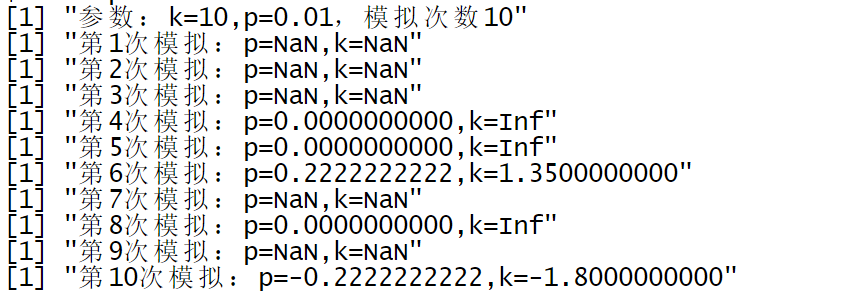
\includegraphics[scale=0.6]{experi1.png}
\end{minipage}
\begin{minipage}{0.5\textwidth}
    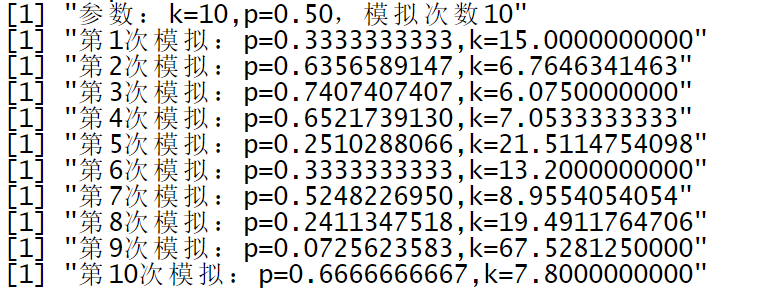
\includegraphics[scale=0.6]{experi2.png}
\end{minipage}
\begin{minipage}{0.5\textwidth}
    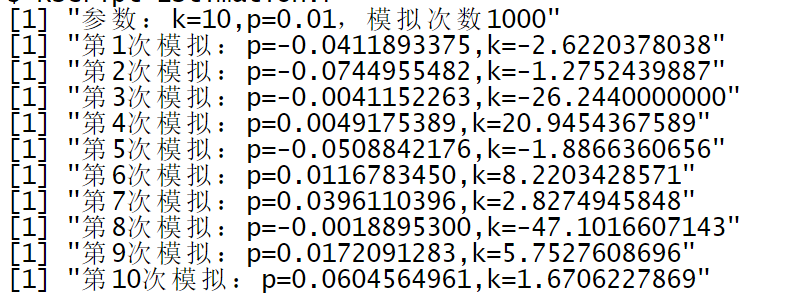
\includegraphics[scale=0.6]{experi3.png}
\end{minipage}
\begin{minipage}{0.5\textwidth}
    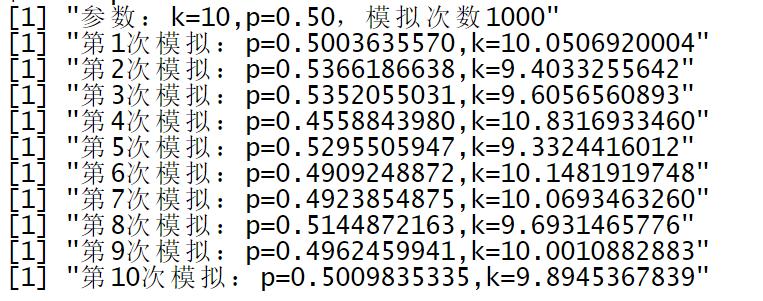
\includegraphics[scale=0.6]{experi4.png}
\end{minipage}
\subsection{问题}
在$p$很小或$n$很小时,很容易得到估计不准的情况,$p$小的时候参数可能会被计算成负值,$n$小的时候虽然不会出现负值但估计也很不准确,而$n,p$都很小的时候甚至会产生数学错误(发生0次时,均值和方差均为0,产生NaN,而发生1次时,$p$的估计值为0,$k$产生Inf)
\\只有$p,n$都足够大的情况下,矩估计才能得到好的估计结果
\end{CJK}
\end{document}